% arara: xelatex: { shell : yes }

% kompilace xelatex prezentace.tex
% dokumentace k beameru: http://ftp.cvut.cz/tex-archive/macros/latex/contrib/beamer/doc/beameruserguide.pdf

\RequirePackage[hyphens]{url}

% nastavení formátu prezentace 16:9 
\documentclass[czech,aspectratio=169]{beamer}

\usepackage{polyglossia}
\setmainlanguage{czech}

% nastavení vzhledu 
% další možnosti vzhledu viz https://hartwork.org/beamer-theme-matrix/
\usetheme{Madrid}
\usecolortheme{whale}

% vzhled slajdů vnitřní téma (např. vzhled odrážek)
\useinnertheme{rectangles} %možnosti: default circles rectangles rounded inmargin
% vzhled slajdů vnější téma
\useoutertheme{default} %možnosti: default, miniframes, smoothbars, sidebar, split, shadow, tree, smoothtree, infolines

% zavedeme čvutí modou barvu
\definecolor{CVUT}{HTML}{0065BD}
% čvutí modou použijeme jako hlavní barvu prezentace
\setbeamercolor{structure}{bg=white,fg=CVUT}

% jako font prezentace nadefinujeme oficiální ČVUT písmo Technika -- pokud chcete použít, musíte si font nainstalovat nebo jej nahrát na Overleaf
% https://www.cvut.cz/logo-a-graficky-manual  -- inforek, přihlášení přes celoškolské heslo
%\usepackage{fontspec}
%\setsansfont{Technika-Kniha}

% vypneme navigační panel beamer (pro zapnutí zakomentujeme)
%\beamertemplatenavigationsymbolsempty

% vygenerujeme slajdy s poznámkami -- ty si můžete vytisknout a mít je na obhajobu s sebou (pokud zapomenete slova, nebo kdyby nefungovalo promítání z nějakého důvodu)
%\setbeameroption{show notes}

% další balíčky
\usepackage{graphicx}
\usepackage{minted}
\usepackage{hyperref}
\usepackage{tikz}
\usetikzlibrary{chains,fit,shapes}

% Údaje o prezentaci
\title[Kooperativní mobilní multiplatformní hra]{Kooperativní mobilní multiplatformní hra}
\subtitle{Bakalářská práce}
\institute[FIT ČVUT v~Praze]{Fakulta informačních technologií \\ České vysoké učení technické v~Praze}
\author[J. Bittner]{Jan Bittner \\ Vedoucí práce: Ing. Marek Suchánek}
\date{30. 6. 2020}
\titlegraphic{
\includegraphics[width=.1\textwidth]{assets/slides/logo-cvut}}

\begin{document}
  \begin{frame}
    \titlepage 
    \note{Nezapomenout pozdravit} %tohle je poznámka, ta na slajdu nebude, ale vygeneruje se vedle něj, pokud odkomentujete příkaz výše -- \setbeameroption{show notes} 
  \end{frame}
  
  %\begin{frame}
  %  \tableofcontents %generuje se automaticky z section, subsection, subsubsection
  %\end{frame}

  \begin{frame}{Motivace volby tématu}
    \begin{center}
      77 \% uživatelů mobilních zařízeních hraje hry.
      \vskip5mm
      Vytvoření mobilní hry pro více platforem\\
      ve formě open-source řešení\\
      se zaměřením na snadnou rozšiřitelnost a~udržitelnost.
    \end{center}
  \end{frame}

  \begin{frame}{Cíle práce}
    \begin{itemize}
      \item analýza podobných aplikací a~trendů
      \item analýza technologií pro vývoj
      \item návrh hry a~herní logiky
      \item návrh a~implementace hry
      \item otestování funkčnosti
    \end{itemize}
  \end{frame}

  \begin{frame}{Technologie}
    \begin{itemize}
      \item \textbf{Flutter} -- multiplatformní framework
      \item \textbf{Bloc} -- knihovna pro správu stavů
      \item \textbf{Clean Architecture} -- architektura
      \item \textbf{Cloud Firestore} -- NoSQL databáze
    \end{itemize}
  \end{frame}

  \begin{frame}{Clean Architecture}
    \begin{center}
      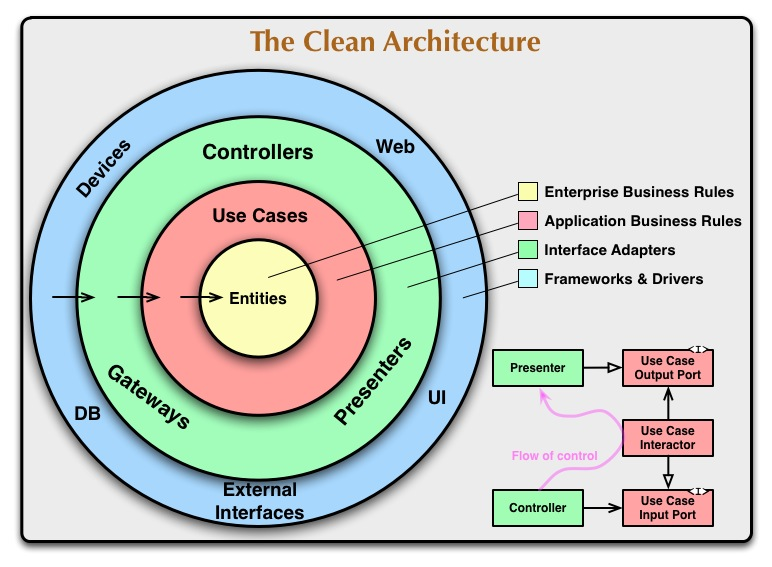
\includegraphics[width=.6\textwidth]{assets/slides/logo-clean-architecture}
    \end{center}
  \end{frame}

  \begin{frame}
      \begin{center}
        {\large ``The way you keep software soft is
      to leave as many options open as possible,
      for as long as possible.
      What are the options that we need to leave open?\\
      They are the details
      that don’t matter.''}
      \vskip5mm
      --- Robert C. Martin, Clean Architecture
      \end{center}
  \end{frame}

  % TODO: upravit obrázek
  \begin{frame}{Návrh hry}
    \begin{center}
      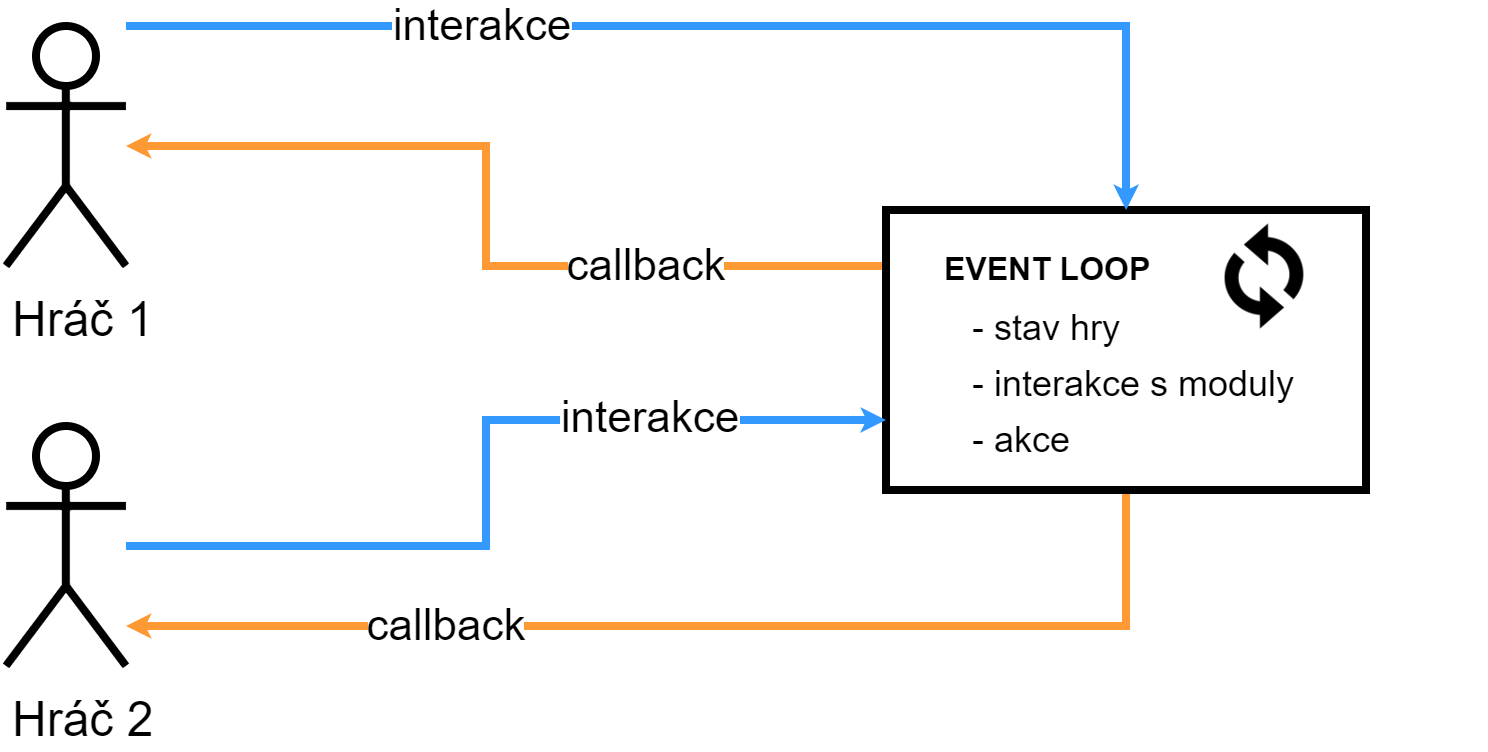
\includegraphics[width=.6\textwidth]{assets/slides/event-loop}
    \end{center}
  \end{frame}

  \begin{frame}
    \begin{columns}
      \begin{column}{.25\textwidth}
        \begin{center}
          
\includegraphics[width=.9\textwidth]{assets/slides/screen-a1}
        \end{center}
      \end{column}
      \begin{column}{.25\textwidth}
        \begin{center}
          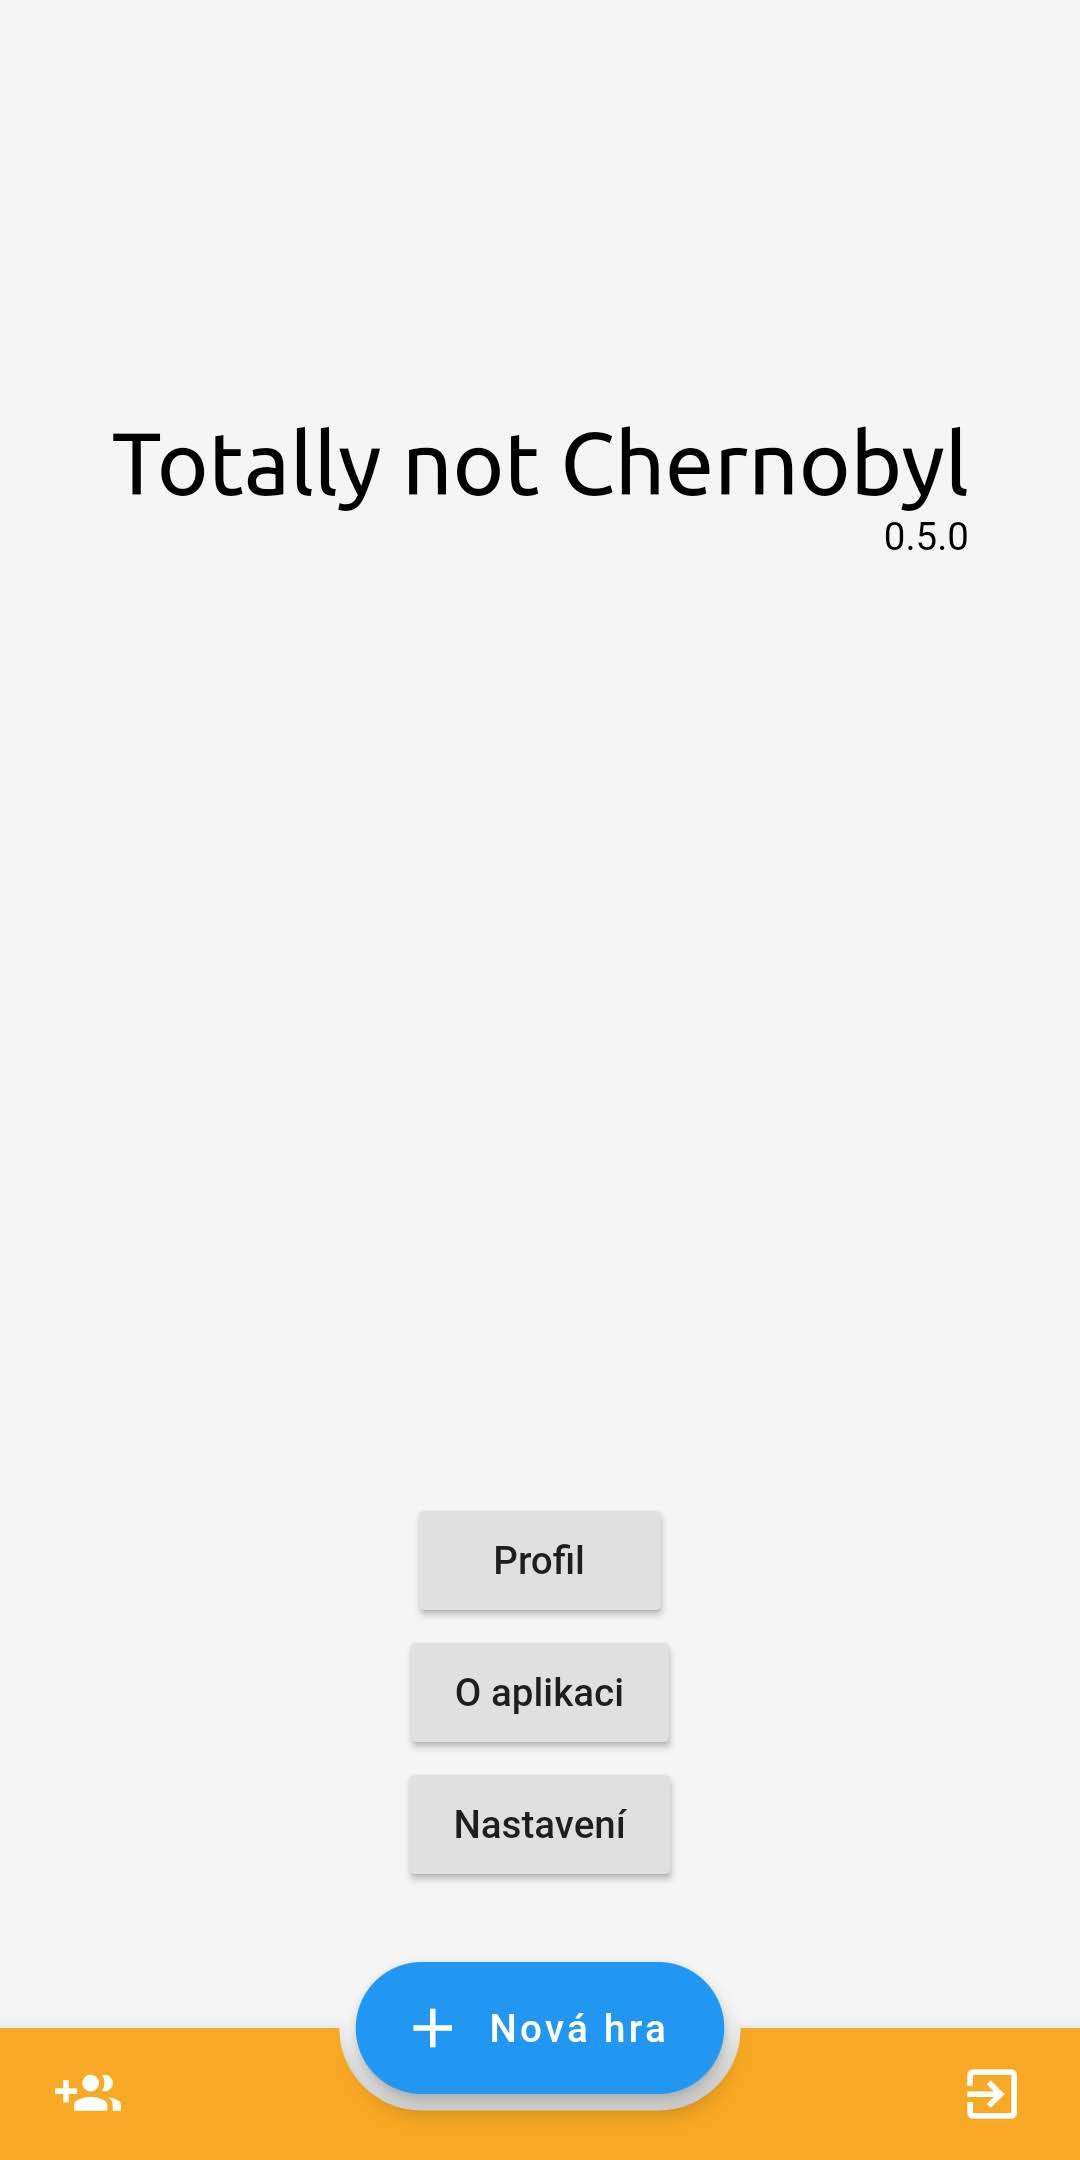
\includegraphics[width=.9\textwidth]{assets/slides/screen-a2}
        \end{center}
      \end{column} 
      \begin{column}{.25\textwidth}
        \begin{center}
          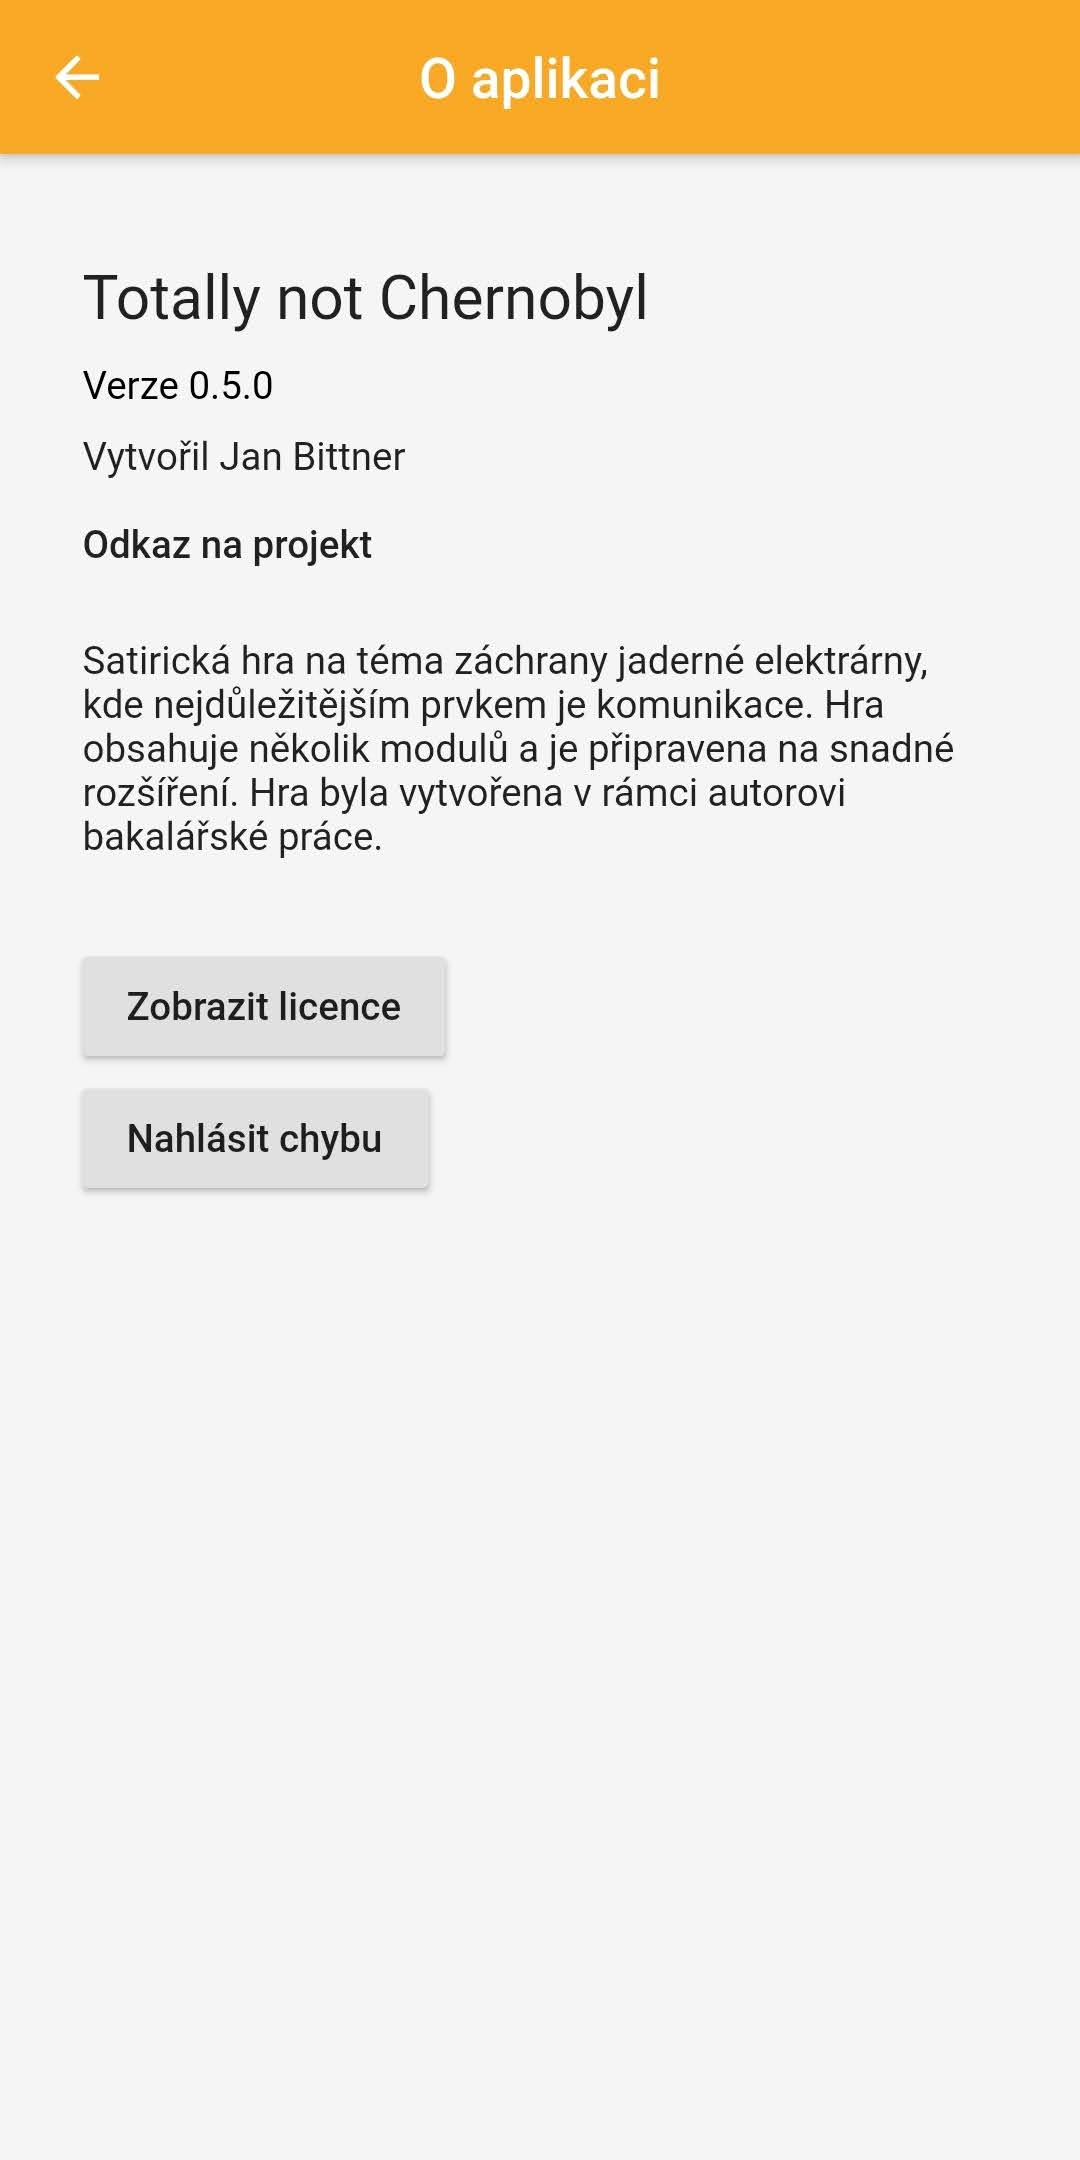
\includegraphics[width=.9\textwidth]{assets/slides/screen-a3}
        \end{center}
      \end{column}
    \end{columns}
  \end{frame}

  \begin{frame}
    \begin{columns}
      \begin{column}{.25\textwidth}
        \begin{center}
          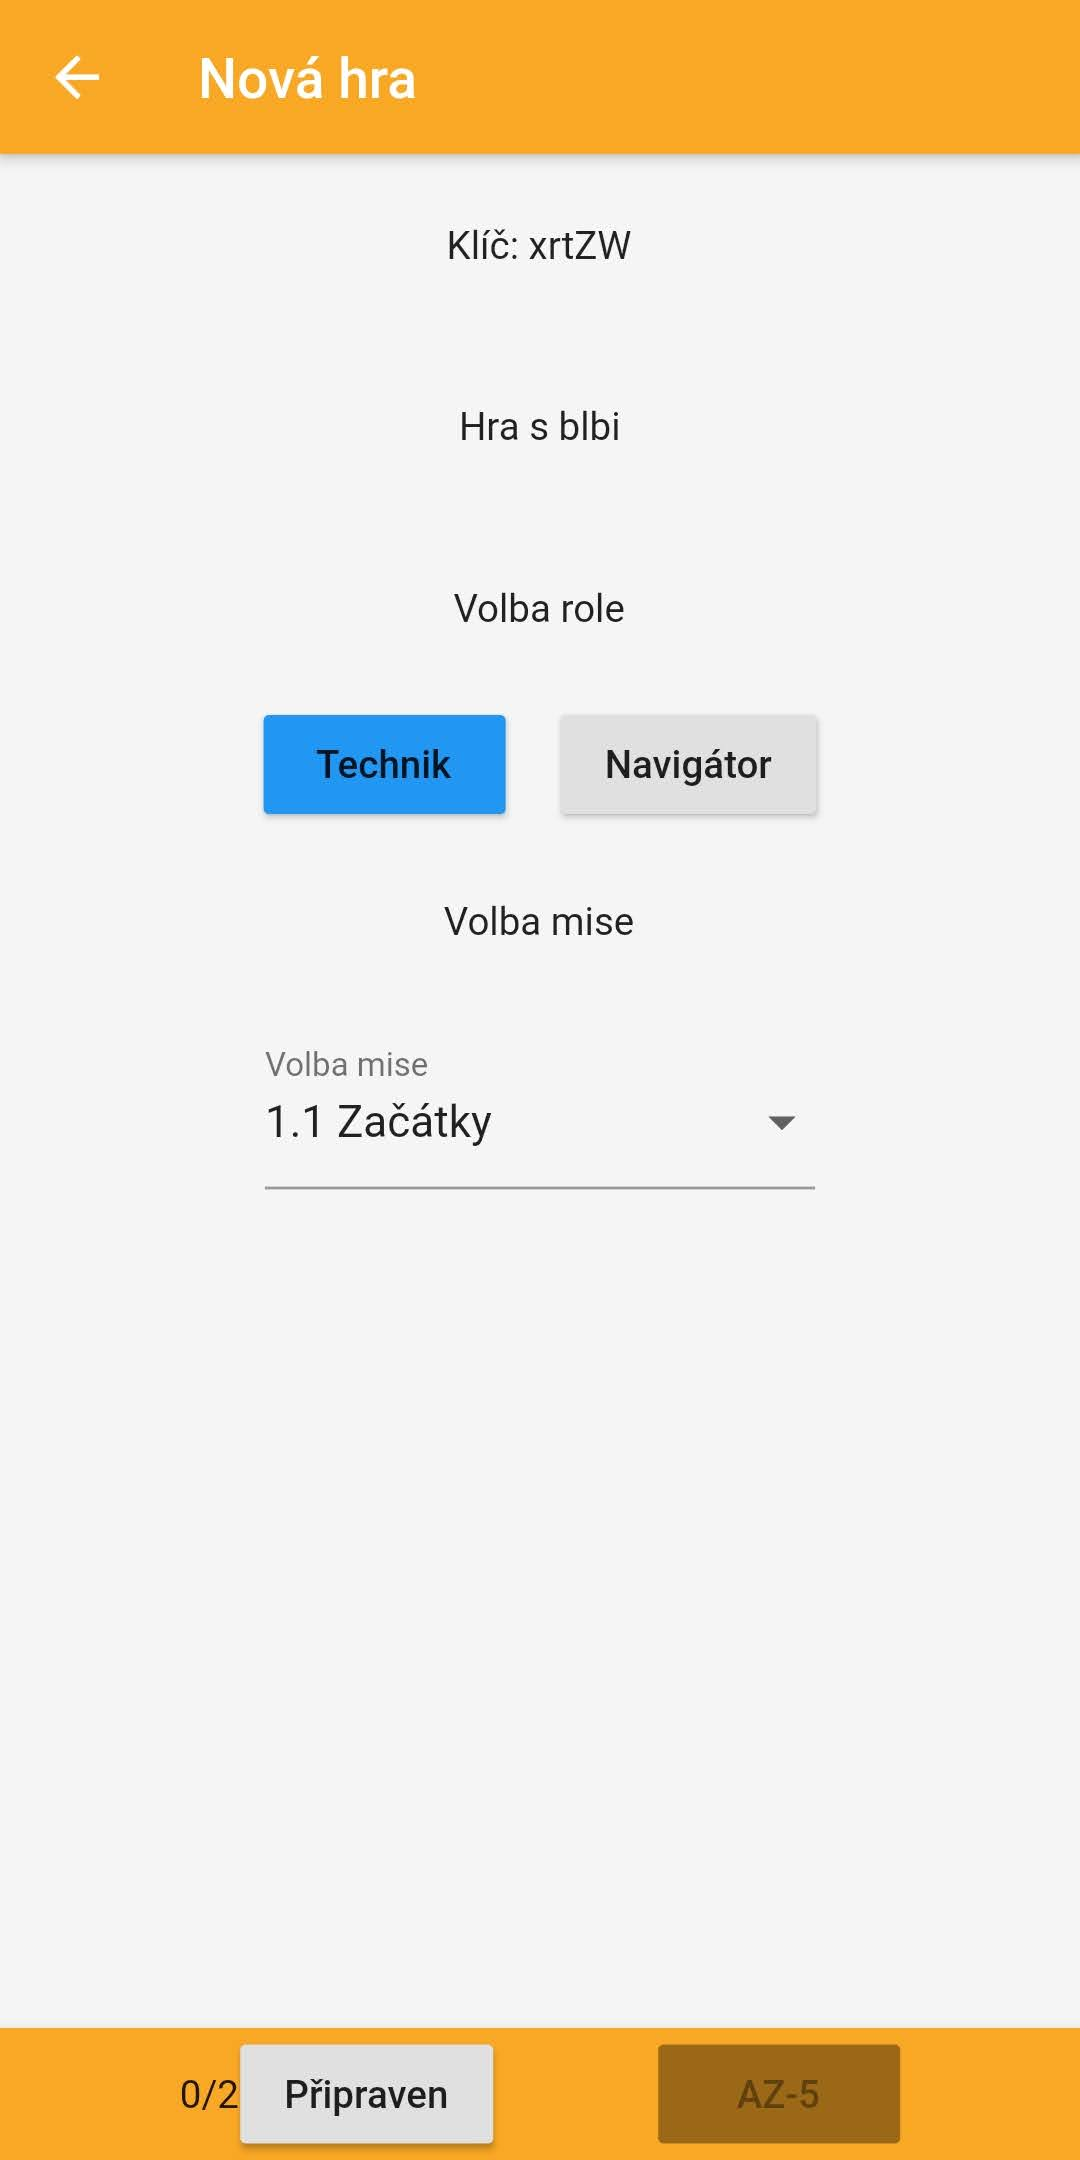
\includegraphics[width=.9\textwidth]{assets/slides/screen-b1}
        \end{center}
      \end{column}
      \begin{column}{.25\textwidth}
        \begin{center}
          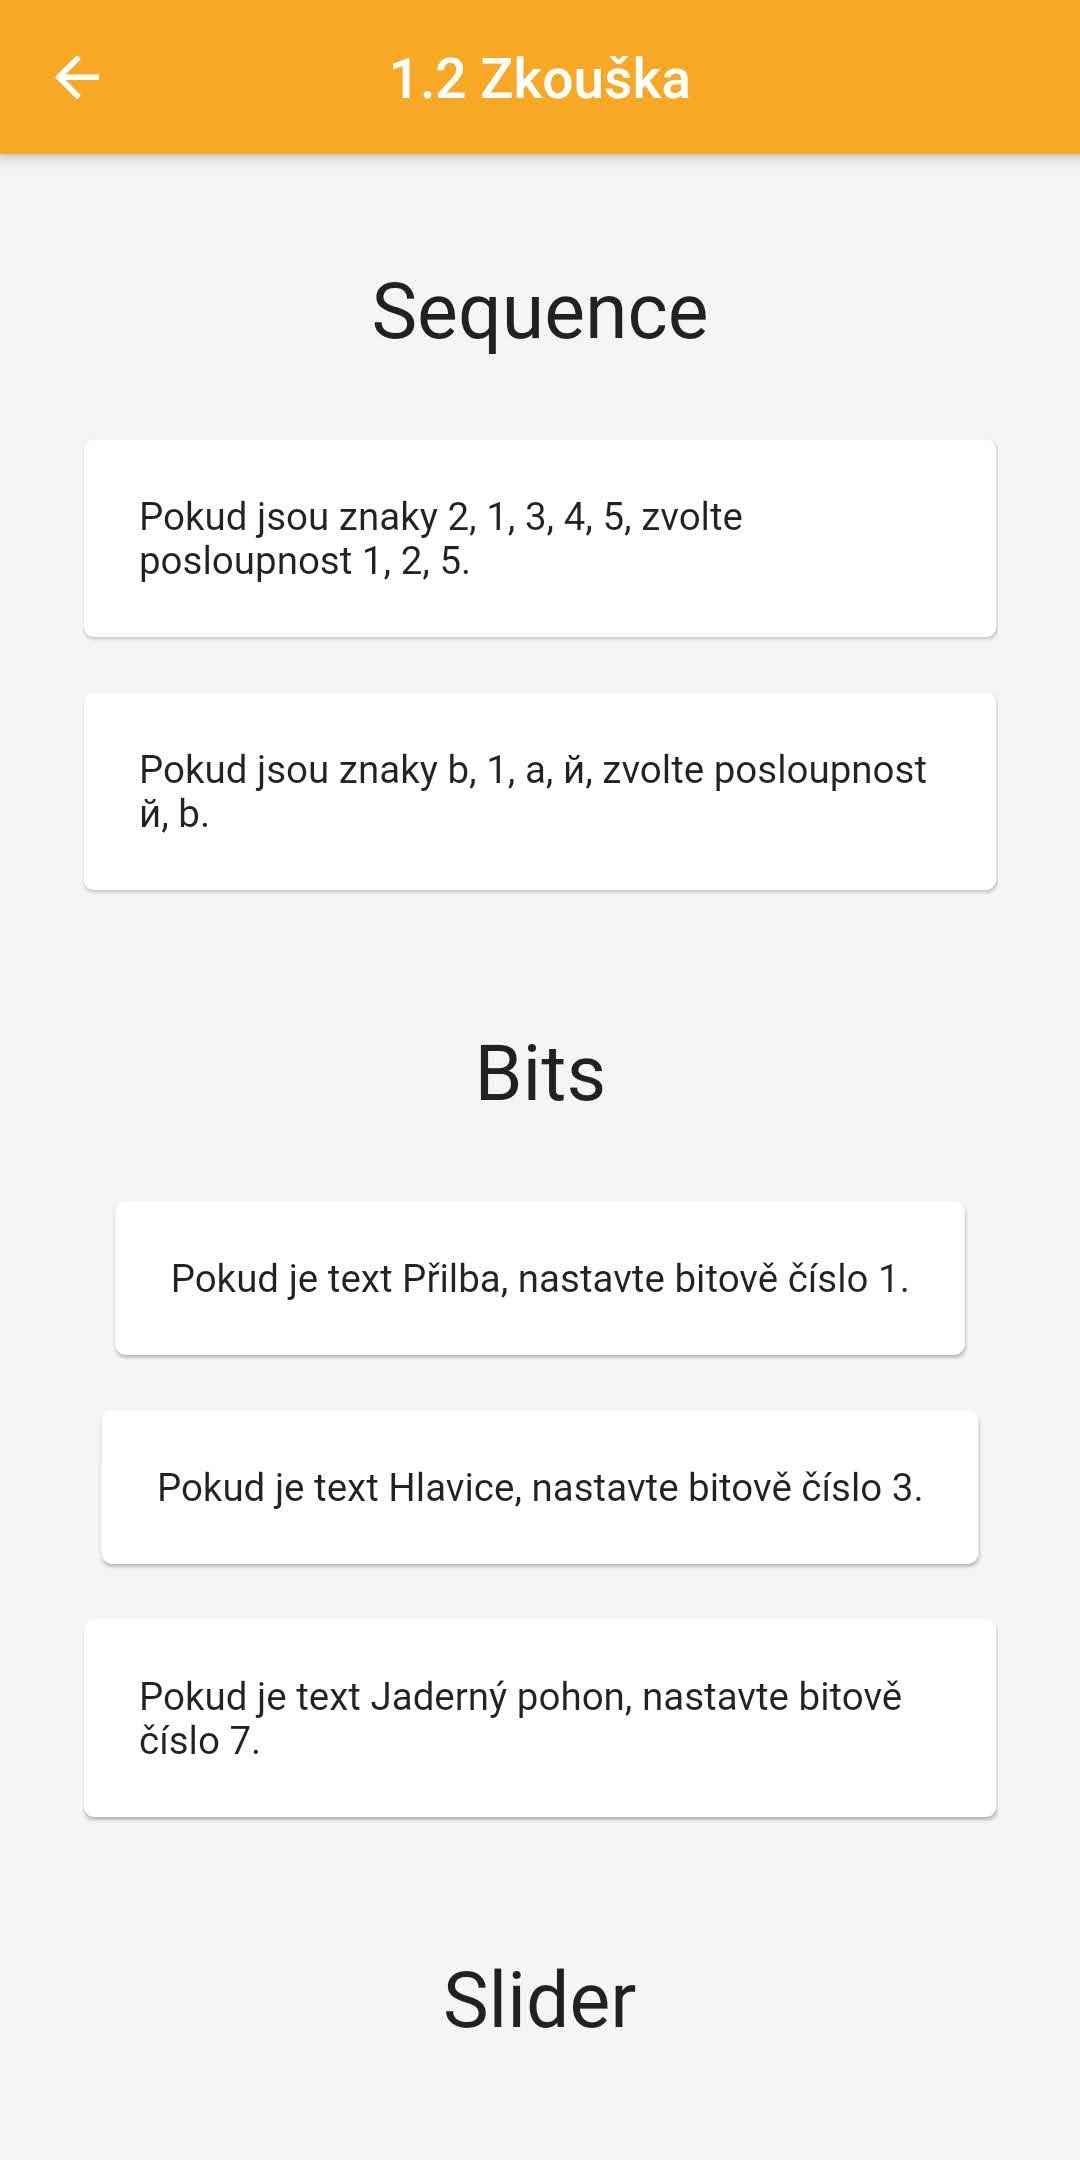
\includegraphics[width=.9\textwidth]{assets/slides/screen-b2}
        \end{center}
      \end{column}
      \begin{column}{.25\textwidth}
        \begin{center}
          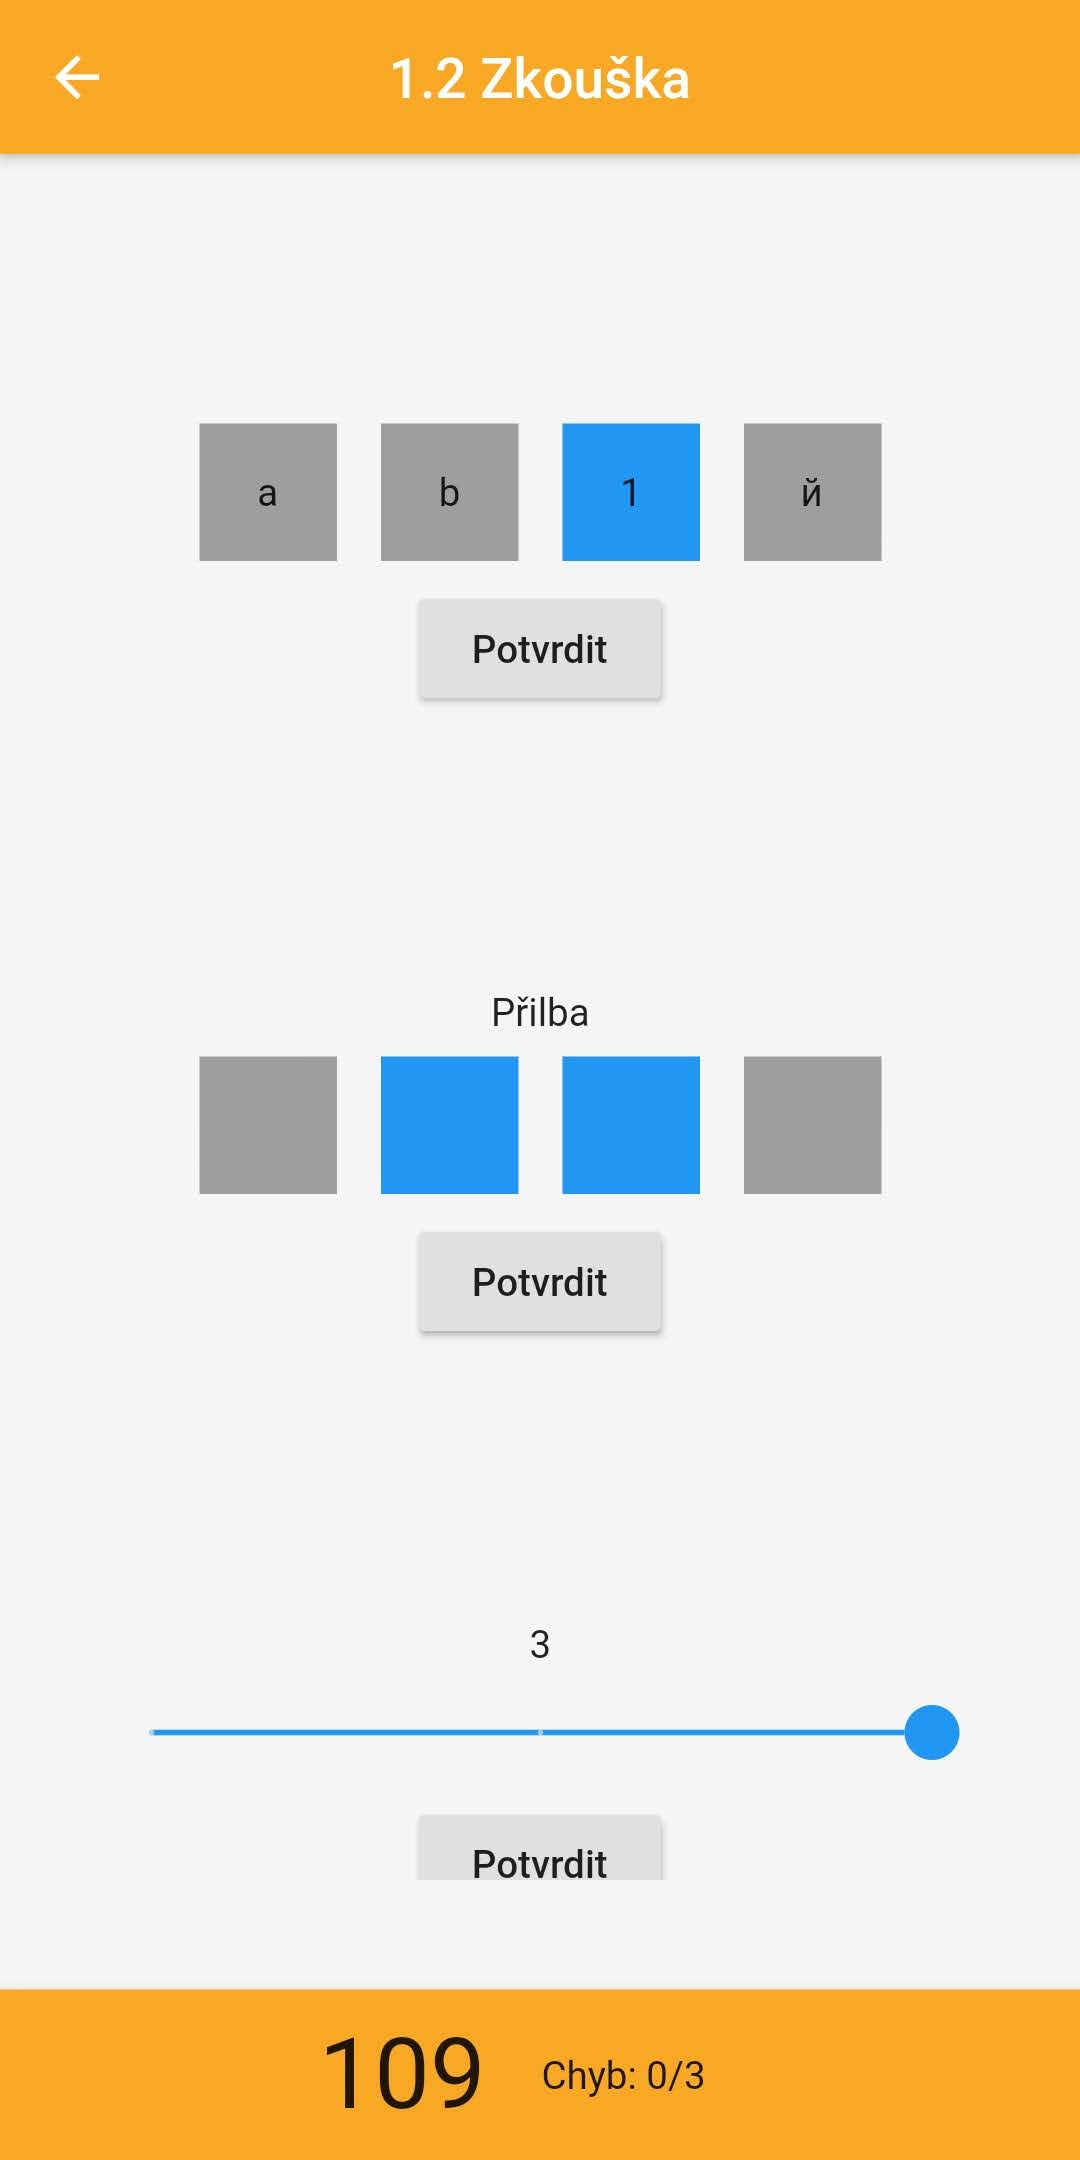
\includegraphics[width=.9\textwidth]{assets/slides/screen-b3}
        \end{center}
      \end{column}
      \begin{column}{.25\textwidth}
        \begin{center}
          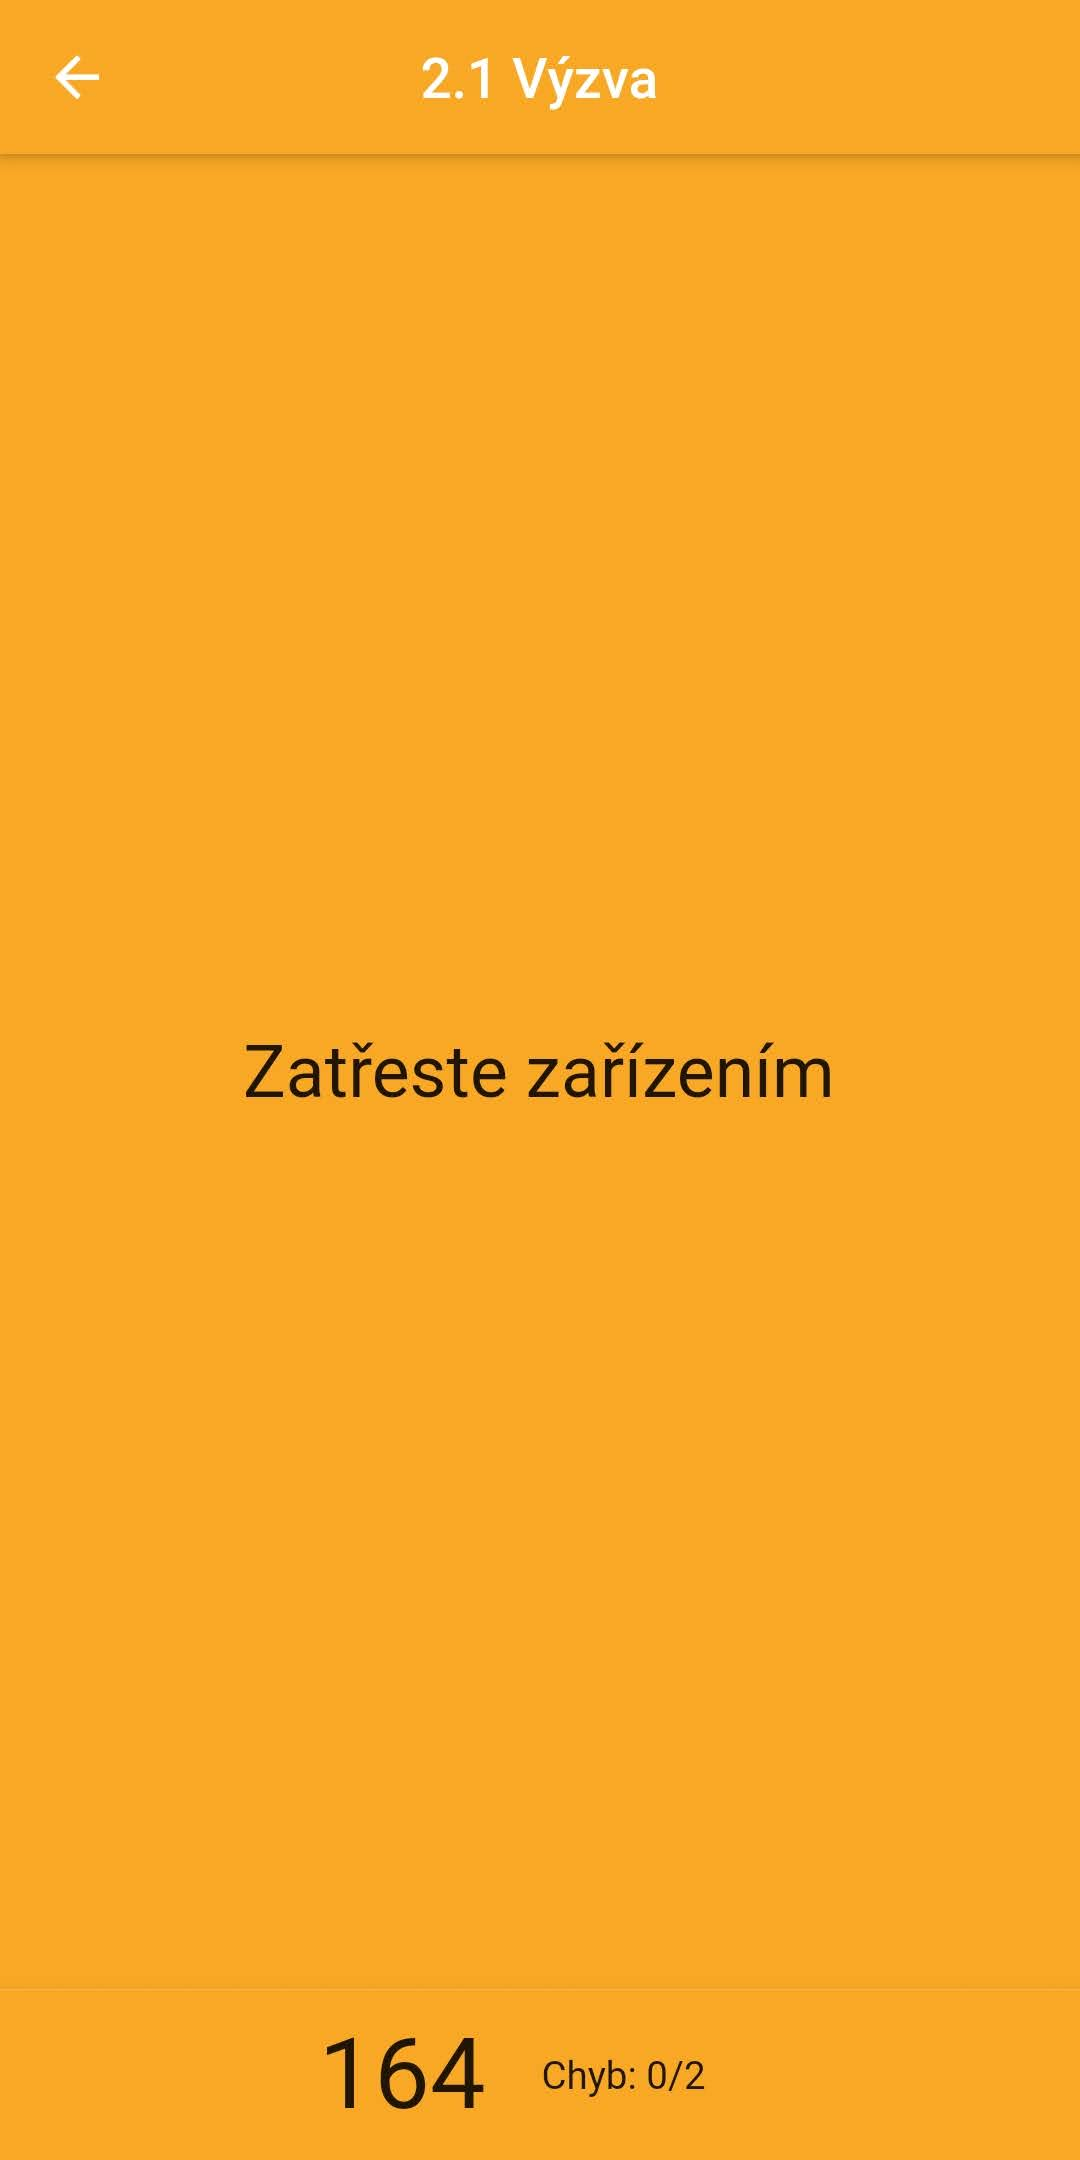
\includegraphics[width=.9\textwidth]{assets/slides/screen-b4}
        \end{center}
      \end{column}
    \end{columns}
  \end{frame}

  \begin{frame}{Shrnutí}
    \begin{itemize}
      \item Všechny cíle splněny.
      \item Úspěšný návrh a~vytvoření funčního řešení hry.
      \item Úspěšné cílení na snadnou rozšířitelnost.
      \item Přínos aplikace pro obohacení komunity Flutter.
      \item Spokojenost uživatelů při testování aplikace.
      \item Mnoho možností rozšíření a~adaptace.
    \end{itemize}
  \end{frame}

  \begin{frame}{Zdroje}
    \begin{itemize}
      \item WEPC. \emph{2020 Video Game Industry Statistics, Trends \& Data} [online]. 2020 [cit. 2020-03-21]. Dostupné z: \url{https://www.wepc.com/news/video-game-statistics}.
      \item MARTIN, Robert C. \emph{The Clean Architecture} [online]. 2012 [cit. 2020-04-07]. Dostupné z: \url{https://blog.cleancoder.com/uncle-bob/2012/08/13/the-clean-architecture.html}.
      \item MARTIN, Robert C. \emph{Clean Architecture: A~Craftsman’s Guide to Soft-ware Structure and Design}. Prentice Hall, 2018, s. 140. ISBN 0134494164. Dostupné z: \url{https://www.amazon.com/Clean-Architecture-Craftsmans-Software-Structure-ebook/dp/B075LRM681}. 
    \end{itemize}
  \end{frame}

  \begin{frame}{Děkuji za pozornost}
    \begin{center}
      Prostor pro dotazy.
    \end{center}
  \end{frame}

  \begin{frame}[noframenumbering]{Otázky oponenta}
    Otázka první:
    V rámci MobX "generování kódu však není nejrychlější" (str. 20),
    proč neprobíhá tedy generování jen jednou (např. kompilací, transpilací)?

    \vfill

    Odpověď: MobX je knihovna pro správu stavů,
    která vyžaduje pro svou funkčnost generovaný kód.
    Objekty knihoven pro správu stavů jsou prostředníkem mezi
    prezentační a aplikační vrstvou.
    Při změnách ve třídách těchto knihoven je nutné opakovaně generovat kód,
    což způsobuje prodlevu mezi rychlým dodáním změn pomocí
    vlasnosti hot reload frameworku Flutter.
  \end{frame}

  \begin{frame}[noframenumbering]{Otázky oponenta}
    Otázka druhá:
    Pokud jsou "data v NoSQL databázích nestrukturovány" (str. 25),
    jak mohou být efektivnější?

    \vfill

    Odpověď:
    NoSQL databáze mohou být v jistých případech efektivnější,
    protože umožňují ukládání dat,
    které nemají předem definovanou strukturu.
    Data se také často ukládají denormalizovaná,
    což umožňuje jejich rychlejší čtení.
    Tyto databáze (například Cloud Firestore) poskytují přívětivé rozhraní
    včetně real time query.
  \end{frame}

  \begin{frame}[noframenumbering]{Otázky oponenta}
    Otázka třetí: Skutečně "všechna zařízení se systémy Android a iOS" (str. 26) obsahují akcelerometr?

    \vfill

    Odpověď:
    V kontextu práce, která je mířená na moderní mobilní zařízení
    (mobily, tablety),
    obsahují všechna (až na teoretickou množinu výjimek)
    zařízení se systémy Android a iOS akcelerometr.
    Tento senzor je totiž velmi univerzální,
    oproti jiným senzorům (gyroskop) šetrný k baterii
    a najde uplatnění v široké řadě běžných procesů uživatele (rotace displeje).
  \end{frame}
\end{document}
